\documentclass[11pt, a4paper, twocolumn]{article}
\usepackage[utf8]{inputenc}
\usepackage{braket}
\usepackage{hyperref}
\usepackage{graphicx}

\title{Résumé stage}
\author{Damien TOQUER}
\date{Mai-Juillet 2021}

\renewcommand*\contentsname{Contenu}

\begin{document}

\maketitle

\tableofcontents

\section{Résolution de l'équation de Schrödinger}
\subsection{Méthode de Crank-Nicolson}
On utilise l'équation de Schrödinger :
\begin{equation}
	i\hbar\frac{\partial\ket{\psi}}{\partial t} = \hat{H}\ket{\psi} = -\frac{\hbar^2}{2m}\nabla^2\ket{\psi}+\hat{V}\ket{\psi}
\end{equation}
On résout par discrétisation du pas d'espace $\psi(q, t) \rightarrow \{\psi^i(t)\}$ et du pas de temps en conservant la condition $\alpha = \frac{\Delta t}{\Delta x^2}\ll1$. L'équation à résoudre s'écrit sous la forme :
\begin{equation}
	\psi^i(t+\Delta t) = e^{-\frac{iH\Delta t}{\hbar}}\psi^i(t)
\end{equation}
Pour simplifier ce calcul, on pourrait réaliser un développement limité de l'exponentielle. On préfère cependant le développement suivant :
\begin{equation}
	e^{-\frac{iH\Delta t}{\hbar}}\approx\frac{1-i\frac{H\Delta t}{2\hbar}}{1+i\frac{H\Delta t}{2\hbar}}
\end{equation}
On résout donc finalement le système suivant :
\begin{equation}
	\left(1+i\frac{H\Delta t}{2\hbar}\right)\psi^i(t+\Delta t) = \left(1-i\frac{H\Delta t}{2\hbar}\right)\psi^i(t)
\end{equation}
Déterminer $\psi^i(t+\Delta t)$ revient donc à résoudre une équation matricielle. On remarque que la matrice $1+i\frac{H\Delta t}{2\hbar}$ est tridiagonale (les termes non diagonaux provenant du Laplacien). On utilise donc une méthode adaptée à cette forme de matrice\footnote{\url{https://en.wikipedia.org/wiki/Tridiagonal_matrix_algorithm}}.
\subsection{Propagation d'un paquet d'onde gaussien libre}
On se place dans le cas $\hat{V} = 0$ et :
\begin{equation}
	\psi(x, t=0) = \left(\frac{1}{2\pi\sigma_0^2}\right)^{\frac{1}{4}}e^{-\frac{x-x_0}{4\sigma_0^2}+i\frac{p_0(x-x_0)}{\hbar}}
\end{equation}
Où $x_0$ est le centre initial de la gaussienne, $p_0$ est l'impulsion initiale d ce centre et $\sigma_0$ et le spreading initial. 

Théoriquement\footnote{Sanz, Á. S., \& Miret-Artés, S. (2013). A Trajectory Description of Quantum Processes. II. Applications: A Bohmian Perspective (Vol. 831). Springer.}, l'évolution temporelle de cette fonction d'onde est :
\begin{equation}
	\psi(x, t) = \left(\frac{1}{2\pi\tilde{\sigma_t}^2}\right)^{\frac{1}{4}}e^{-\frac{x-x_t}{4\sigma_0\tilde{\sigma_t}}+i\frac{p_0(x-x_t)+E_0t}{\hbar}}
\end{equation}
Où $x_t = x_0 = \frac{p_0}{m}t$, $p_t = p_0$, $E_0 = \frac{p_0^2}{2m}$ est l'énergie totale et :
\begin{equation}
	\tilde{\sigma_t} = \sigma_0\left(1+i\frac{\hbar t}{2m\sigma_0^2}\right)
\end{equation}
Correspond à l'évolution temporelle du spreading.

La figure 1. montre les résultats obtenus par la méthode de Crank-Nicolson.
\begin{figure}
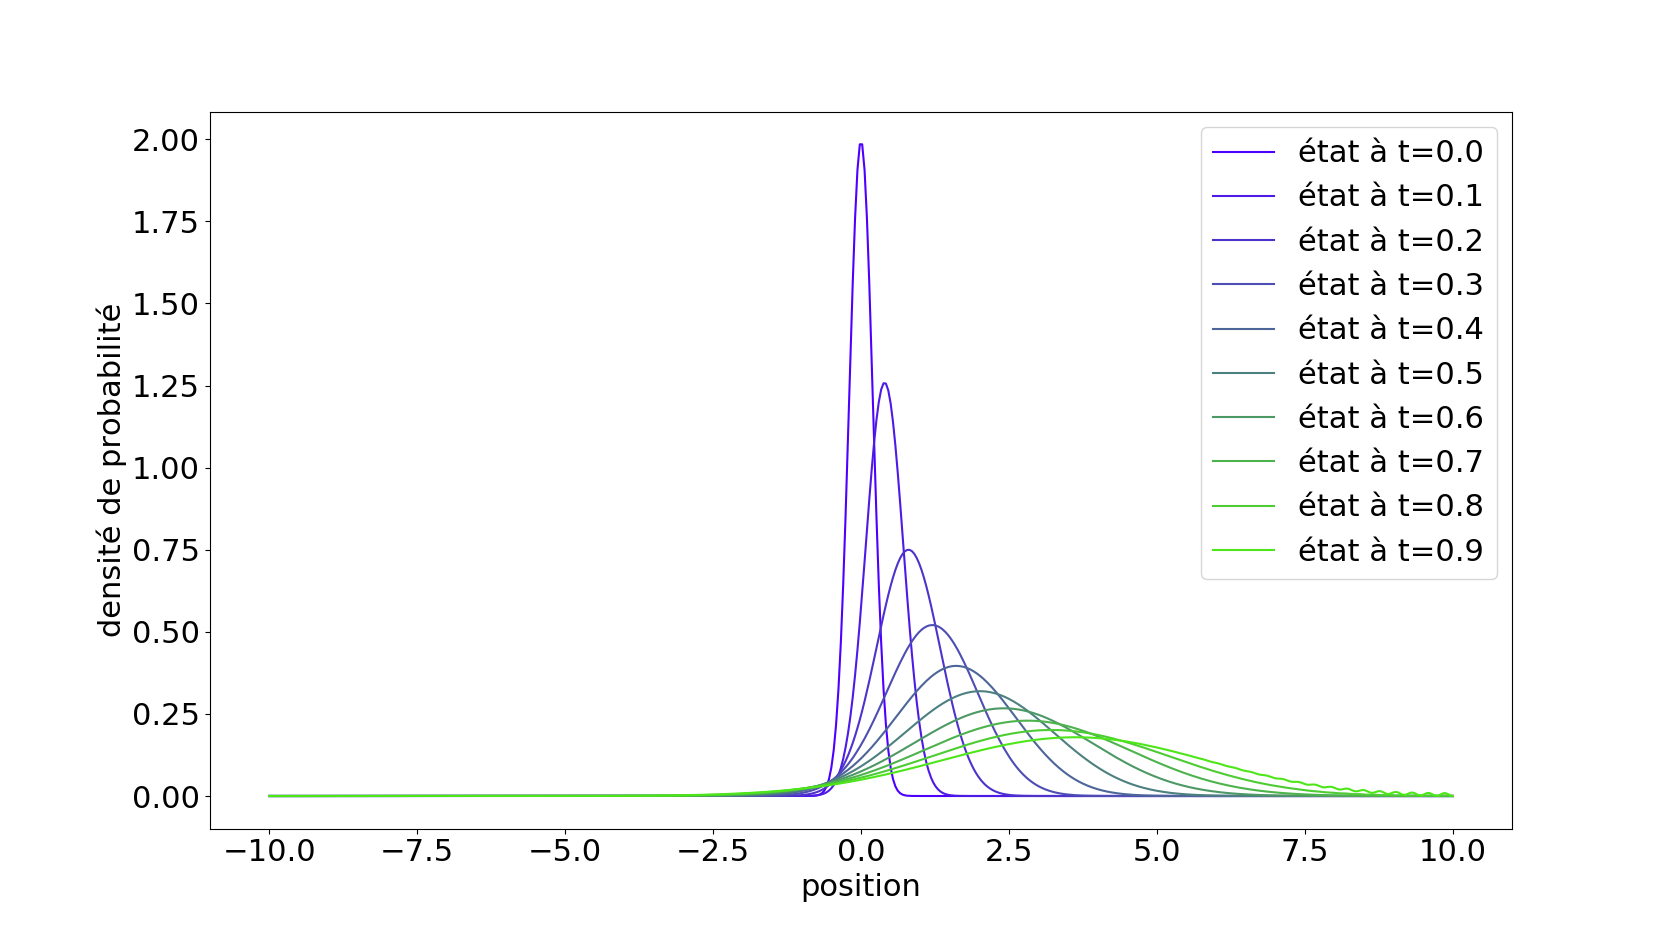
\includegraphics[width=\linewidth]{Figure_1.png}
\caption{Evolution du paquet gaussien avec $\hbar = m = 1$, $x_0 = 0$, $p_0 = 4$, $\sigma_0 = 0.2$ et $\alpha = 0.06$}
\end{figure}
On observe comme prévu une évolution linéaire (potentiel constant) de la position du centre de la gaussienne, et une augmentation du spreading.

Lorsque l'on se rapproche des limites spatiale du système, on observe l'apparition d'oscillation due aux conditions aux limites (dérivée spatiale nulle). On évitera par la suite d'atteindre les limites du domaines.

On peut aussi calculer à l'aide d'intégration numérique la valeur des premiers moments de notre distribution. La figure 1 montre les moments d'ordre 0, 1 et 2 correspondent respectivement à l'intégrale de la densité, la moyenne et la variance.
\begin{figure}
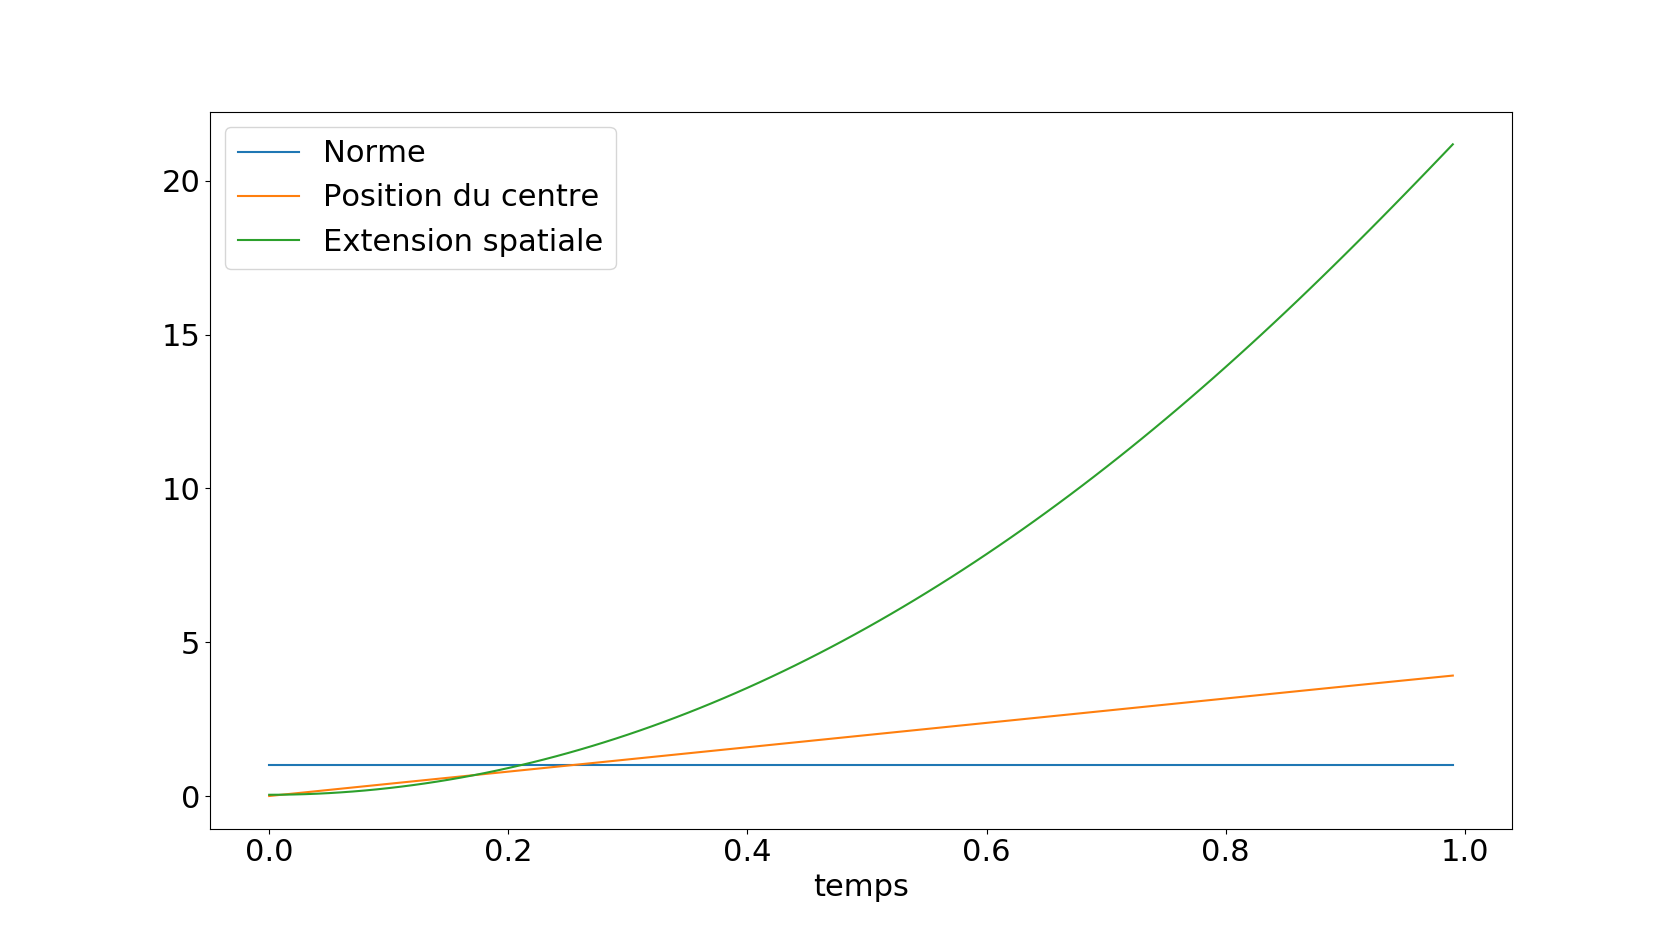
\includegraphics[width=\linewidth]{Figure_2.png}
\caption{3 premiers moments de notre distribution en fonction du temps.}
\end{figure}

Comme attendu par la théorie, le moment d'ordre 0 vaut 1 (intégrale d'une densité de probabilité), le moment d'ordre 1, correspondant à la moyenne se déplace à une vitesse constante et le comportement de la variance est initialement constant (régime de Ehrenfest-Huygens), puis quadratique (régime de Fresnel) et finalement linéaire (régime de Fraunhoffer).

La figure 3 compare finalement les courbes obtenus avec les courbes théorique dérivées analytiquement. On remarque un léger décalage entre les 2 courbes pour $t\neq0$ ce qui justifie l'utilisation plus tard d'une méthode plus précise.
\begin{figure}
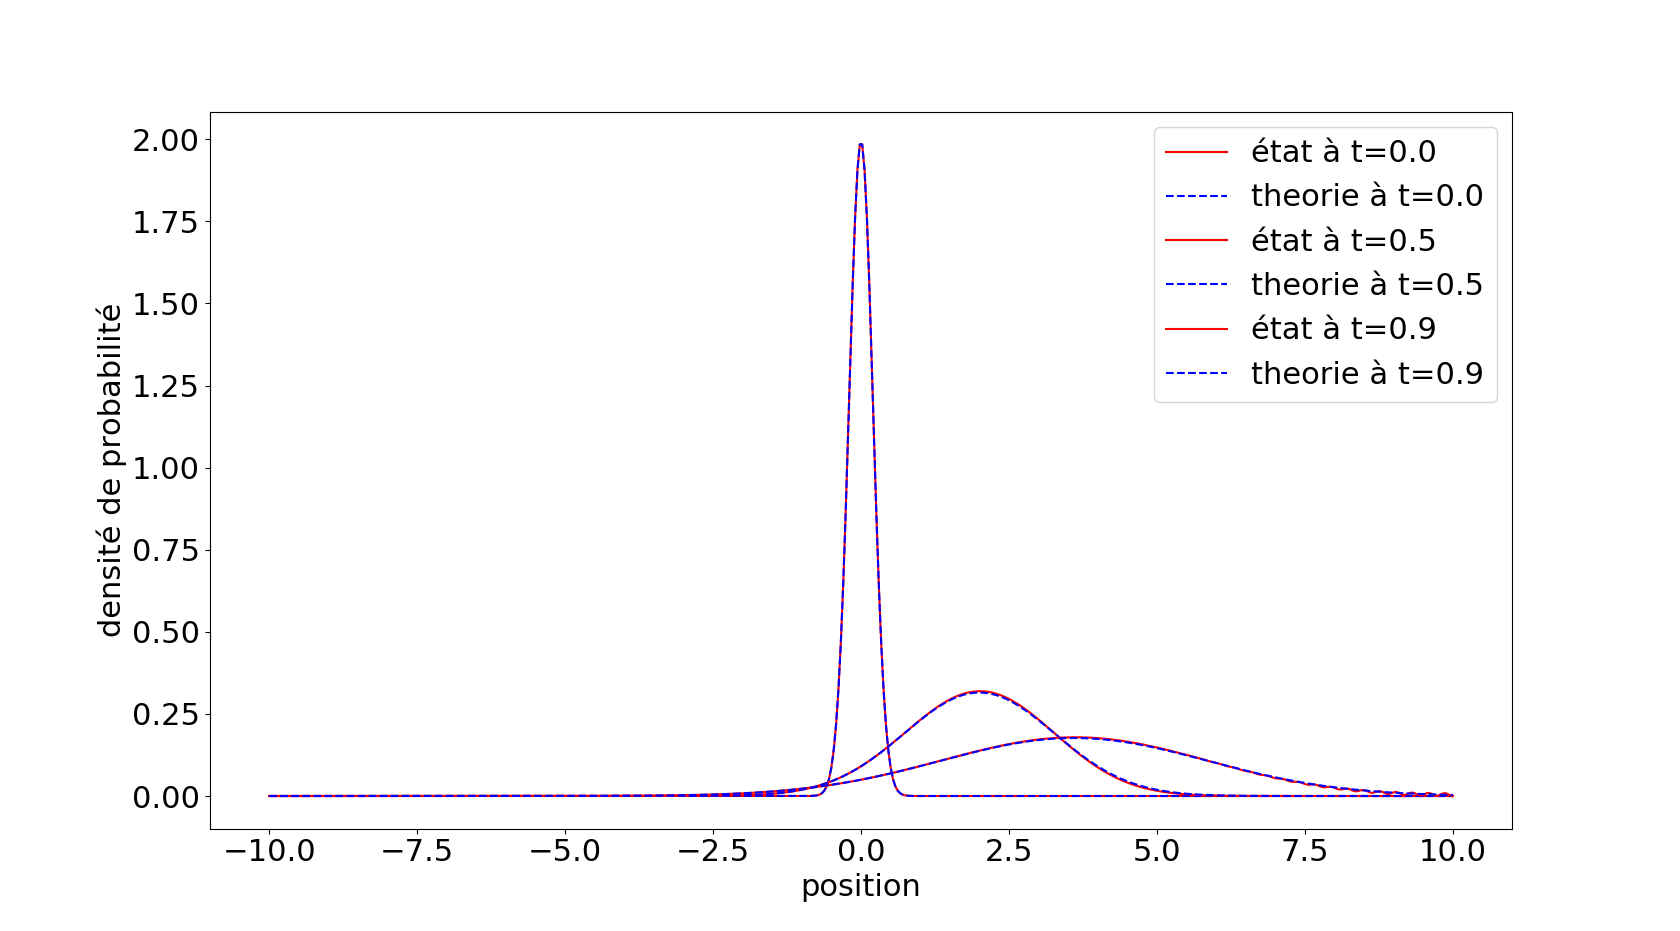
\includegraphics[width=\linewidth]{Figure_3.png}
\caption{Comparaison des courbes obtenus avec la méthode de Crank-Nicolson avec les courbes théoriques.}
\end{figure}
\subsection{Propagation d'un paquet d'onde gaussien non libre}
\subsubsection{Potentiel harmonique}
On se place dans le cas $\hat{V} = \frac{1}{2}m\omega^2\hat{x}^2$. La figure 4 montre l'évolution temporelle du paquet d'onde gaussien tandis que la figure 5 montre l'évolution temporelle des 3 premiers moments de notre distribution.
\begin{figure}
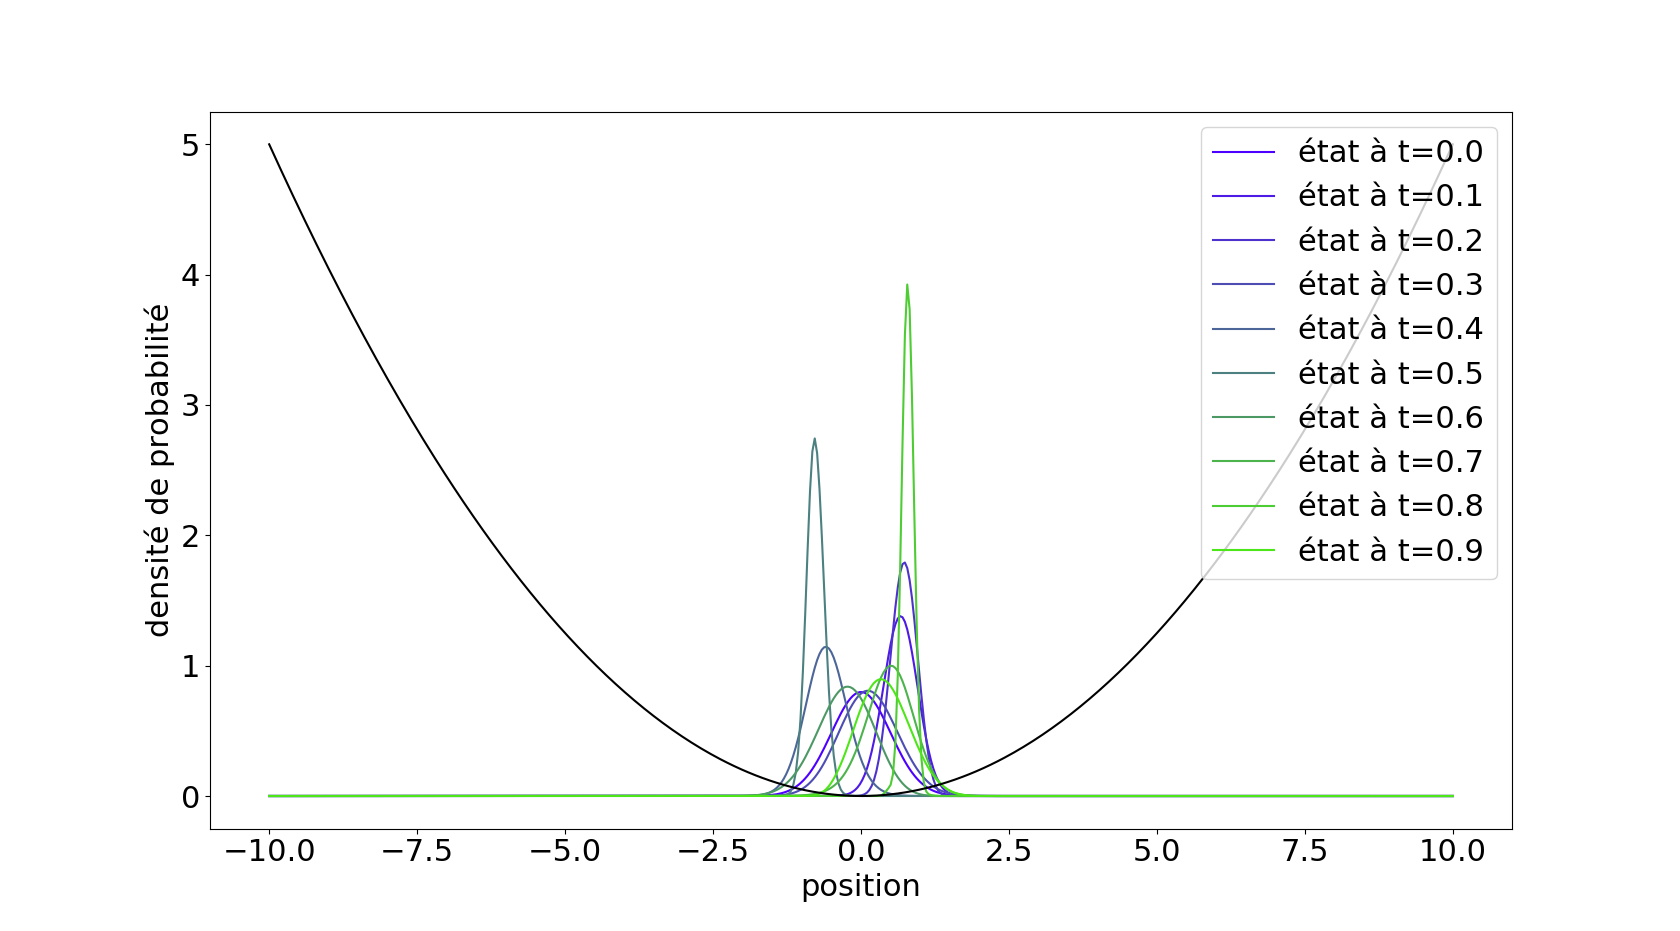
\includegraphics[width=\linewidth]{Figure_4.png}
\caption{Fonction d'onde dans un potentiel harmonique, $\hbar = m = 1$, $x_0 = 0$, $p_0 = 8$, $\sigma_0 = 0.5$, $\omega = 10$ et $\alpha = 0.06$.}
\end{figure}
Le centre de notre distribution oscille dans notre potentiel. On remarque aussi qu'il n'y a pas de diffusion de notre distribution en moyenne.
\begin{figure}
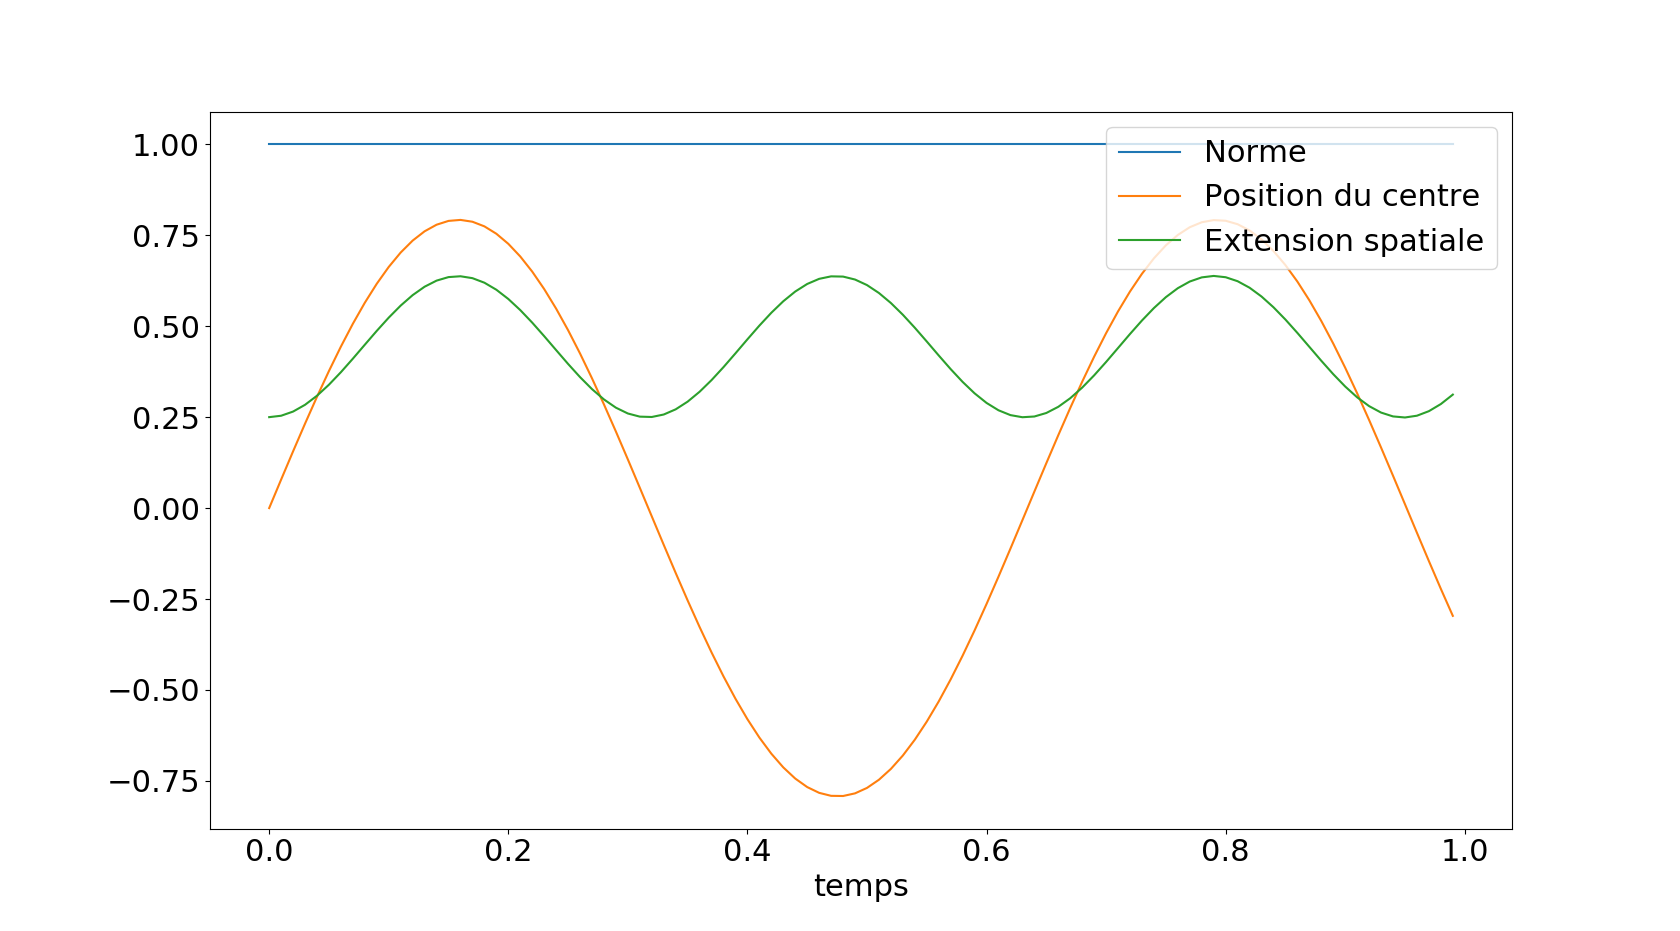
\includegraphics[width=\linewidth]{Figure_5.png}
\caption{3 premiers moments de notre distribution en fonction du temps.}
\end{figure}

\subsection{Méthode du split-operator}
On part encore de :
\begin{equation}
	\psi(x, t+\Delta t) = e^{-i\frac{\hat{H}\Delta t}{\hbar}}\psi(x, t)
\end{equation}
Avec $\hat{H} = \frac{\hat{p}^2}{2m} + \hat{V}(\hat{x}) = \hat{H}_p+\hat{V}$. Ces 2 termes ne commutant pas, on ne peux pas directement séparer l'exponentielle complexe, mais on peut faire l'approximation suivant :
\begin{equation}
	e^{-i\frac{\hat{H}\Delta t}{\hbar}}\approx e^{-i\frac{\hat{V}\Delta t}{2\hbar}}e^{-i\frac{\hat{H}_p\Delta t}{\hbar}}e^{-i\frac{\hat{V}\Delta t}{2\hbar}}
\end{equation}
Les exponentielles de matrice ayant une forme simple lorsque diagonale, la solution pour ce calcul est de réaliser une transformée de Fourier spatiale (fft) pour calculer l'exponentielle d'impulsion.

\end{document}